\def\mySecNum{2.1}
\mySection{\mySecNum~Forward contracts}
%-------------- start slide -------------------------------%{{{ 1
\begin{frame}[fragile,t]
	\begin{mydefinition}
		\textcolor{magenta}{Forward contract} is a binding agreement (obligation) to buy or sell an
		underlying asset in the future, at a price set today.  The time at which the contract settles is
		called the \textcolor{magenta}{expiration date}.  A forward contract specifies
		\begin{itemize}
			\item The features and quantity of the asset to be delivered.
			\item The delivery logistics, such as time, date, and place.
			\item The price the buyer will pay at the time of delivery.
		\end{itemize}
	\end{mydefinition}
	\bigskip
	\begin{remark}
		\begin{enumerate}
			\item \textcolor{magenta}{Futures contracts} are the same as forwards in principle except for
				some institutional and pricing differences. We will study future contracts in Chapter 5.
			\item A forward contract requires no initial payment or \textcolor{magenta}{premium}.
		\end{enumerate}
	\end{remark}
\end{frame}
%-------------- end slide -------------------------------%}}}
%-------------- start slide -------------------------------%{{{ 1
\begin{frame}[fragile,t]
	\begin{center}
		\textcolor{green}{Long} = buy \qquad \textcolor{red}{short} = sell
	\end{center}

	\bigskip
	\begin{mydefinition}
		\textcolor{magenta}{Payoff for a contract} is its value at expiration. In particular, for
		forward contracts,
		\bigskip
		\begin{center}
			Payoff for \textcolor{green}{Long} forward = Spot price at expiration $-$ Forward price \\ \bigskip
			Payoff for \textcolor{red}{Short} forward = Forward price $-$ Spot price at expiration
		\end{center}
	\end{mydefinition}
	\vfill

	\begin{remark}
		Payoff and \textcolor{magenta}{profit (net payoff)} are the same for forward contracts because
		there is no initial payment -- \textcolor{cyan}{premium}.
	\end{remark}
\end{frame}
%-------------- end slide -------------------------------%}}}
%-------------- start slide -------------------------------%{{{ 1
\begin{frame}[fragile,t]
	\begin{myexample}
	  S\&R (special and rich) index:
		\begin{center}
			Today: Spot price = \$1,000\\
			6-month forward price = \$1,020 \\
			In six months at contract expiration: Spot price = \$1,050.
		\end{center}
		What are the payoff of long/short forward?
	\end{myexample}
	\bigskip
	\pause
	\begin{mysol}
		\begin{center}
		Long position payoff $=\$1,050-\$1,020 = \$30$, \\ \bigskip
		Short position payoff $= \$1,020-\$1,050 = (\$30)$.
		\end{center}
		\myEnd
	\end{mysol}
\end{frame}
%-------------- end slide -------------------------------%}}}
%-------------- start slide -------------------------------%{{{ 1
\begin{frame}[fragile,t]
	% \frametitle{Payoff diagram for forwards}
\begin{center}
	Payoff diagram for a forward price = \$1,020 \\
	\bigskip

	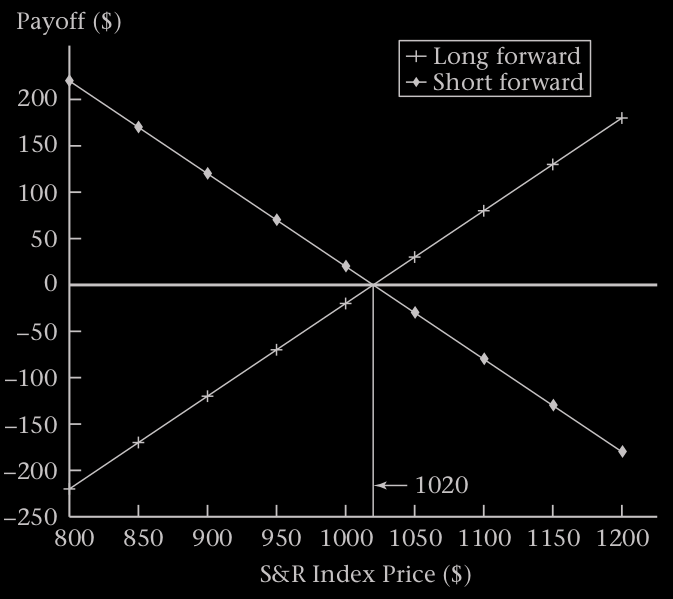
\includegraphics[scale=0.2]{figs/Figure-2-2.png}
\end{center}
\end{frame}
%-------------- end slide -------------------------------%}}}
%-------------- start slide -------------------------------%{{{ 1
\begin{frame}[fragile,t]
	\frametitle{Forward versus outright purchase}
	We will see this through the following example:

	\begin{myexample}
		S\&R 6-month forward contract with a zero-coupon bound (e.g., Treasury bills).
		The 6-month interest rate is $2\%$. Spot price today $= \$1,000$.
	\end{myexample}
\end{frame}
%-------------- end slide -------------------------------%}}}
%-------------- start slide -------------------------------%{{{ 1
\begin{frame}[fragile,t]
	\begin{center}
		\$1,000 today is worth $\$1,000 \times 1.02 = \$1,020$ in 6 months.

	\bigskip
	\mySeparateLine
	\bigskip

	\textcolor{magenta}{Outright purchase}\footnote{It is also called \textcolor{magenta}{long physical index}.} is equivalent to
	\textcolor{cyan}{forward + bond}\footnote{Invest \$1,000 to bond for 6 month and enter long
	position of forward contract at the same time.}\\

	\bigskip
	because\\
	\bigskip

	\begin{align*}
		\text{Payoff of \textcolor{cyan}{forward+bond}} & = \underbrace{\text{Spot price at expiration} - \$1,020}_{\text{Forward payoff}} + \underbrace{\$1,020}_{\text{Bound payoff}} \\
                                                    & = \text{Spot price at expiration}                                                                                             \\
																										& = \text{Payoff of \textcolor{magenta}{outright purchase}}
	\end{align*}
	% \bigskip
  %
	% 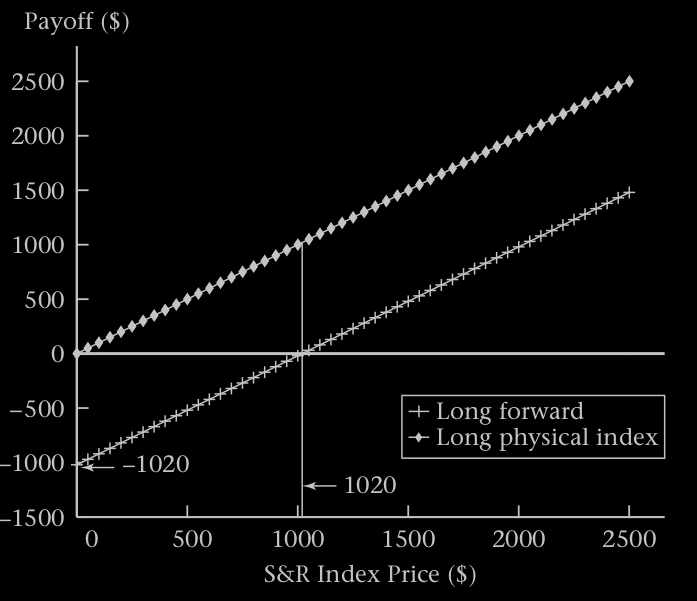
\includegraphics[scale=0.2]{figs/Figure-2-3.png}
	% 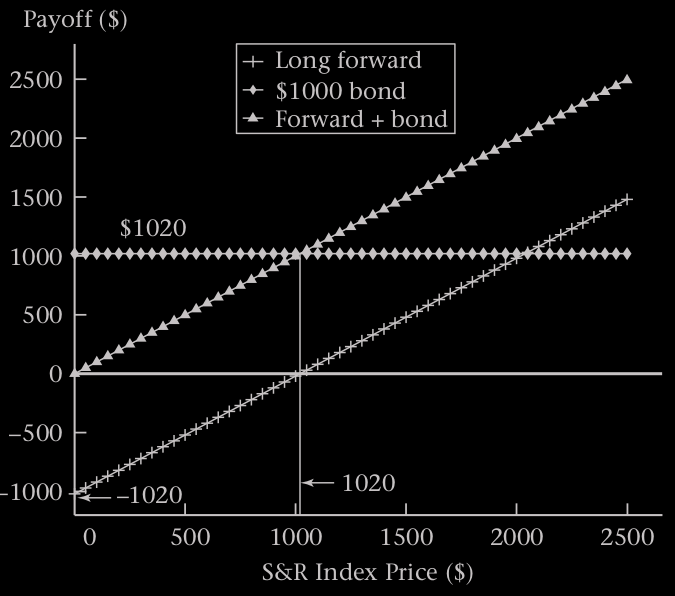
\includegraphics[scale=0.2]{figs/Figure-2-4.png}

	% \bigskip
	\end{center}
\end{frame}
%-------------- end slide -------------------------------%}}}
%-------------- start slide -------------------------------%{{{ 1
\begin{frame}[fragile,t]
	\begin{center}
		\$1,000 today is worth $\$1,000 \times 1.02 = \$1,020$ in 6 months.

	\bigskip
	\mySeparateLine
	\bigskip

	\textcolor{magenta}{Long forward} is equivalent to
	\textcolor{cyan}{borrow-to-buy}\footnote{Borrow money (\$1,000) to outright buy physical index and at expiration
	pay back the money (\$1,020).}

	\bigskip
	because\\
	\bigskip


	\begin{align*}
		\text{Payoff of \textcolor{cyan}{borrow-to-buy}} & = \underbrace{\text{Spot price at expiration}}_{\text{Payoff for outright buy}} - \underbrace{\$1,020}_{\text{Return borrowed money}} \\[1em]
																										 & = \text{Payoff of \textcolor{magenta}{long forward}}.
	\end{align*}

	% \bigskip
  %
	% 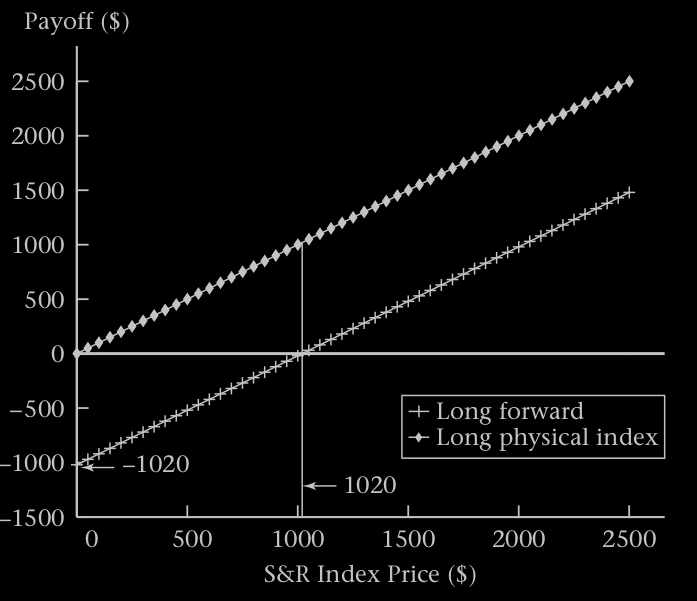
\includegraphics[scale=0.2]{figs/Figure-2-3.png}
	% 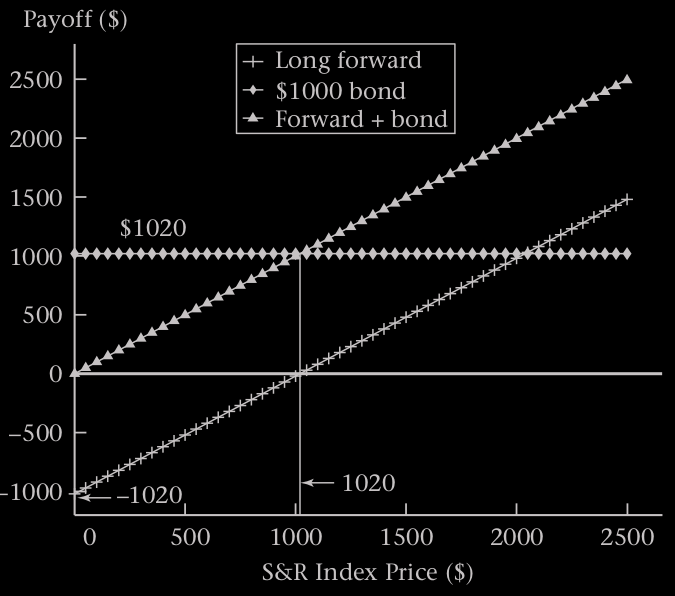
\includegraphics[scale=0.2]{figs/Figure-2-4.png}

	% \bigskip
	\end{center}
\end{frame}
%-------------- end slide -------------------------------%}}}
%-------------- start slide -------------------------------%{{{ 1
\begin{frame}[fragile]
\begin{center}
	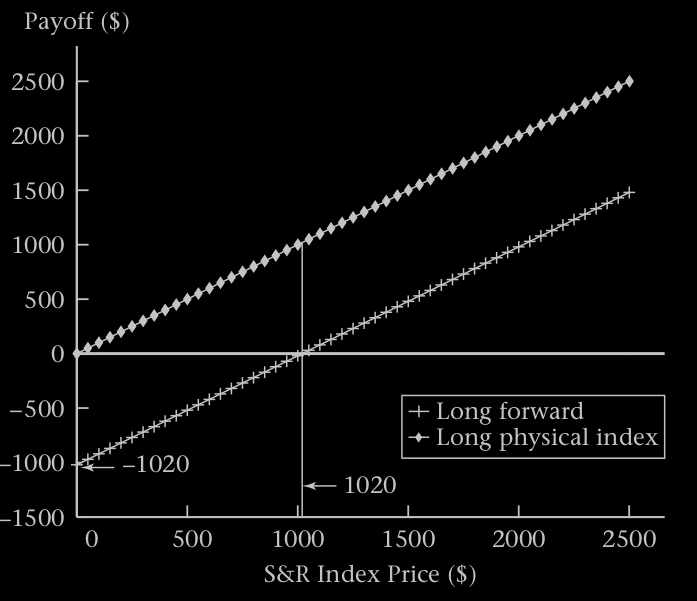
\includegraphics[scale=0.2]{figs/Figure-2-3.png}
	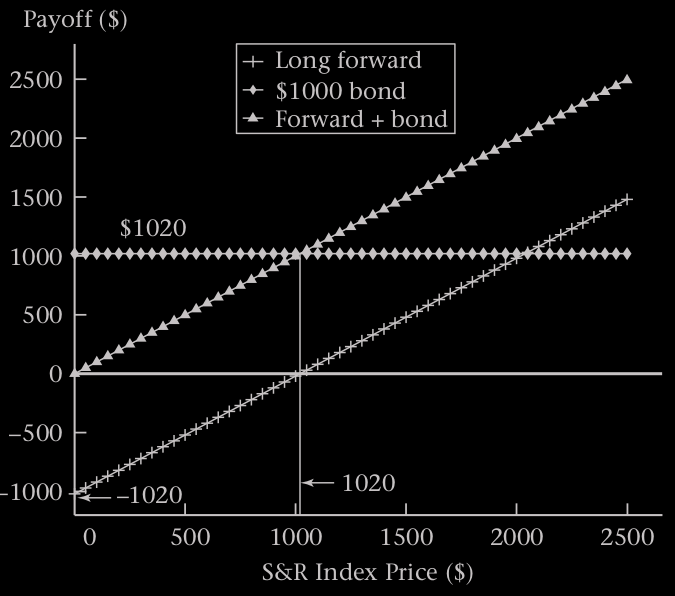
\includegraphics[scale=0.2]{figs/Figure-2-4.png}
\end{center}
\end{frame}
%-------------- end slide -------------------------------%}}}
%-------------- start slide -------------------------------%{{{ 1
\begin{frame}[fragile,t]
	\frametitle{Cash settlement versus physical delivery \\[0.5em]  -- Type of settlement}

	\begin{itemize}
		\item Cash settlement: less costly and more practical
		\item Physical delivery: often avoided due to significant costs
	\end{itemize}
	\bigskip
	\bigskip
	\pause

	\begin{myexample}
		Consider the S\&R index with the forward price \$1,020.\\
		\bigskip

		\begin{itemize}
			\item Suppose that the S\&R index at expiration is \$1,040.
			\item The long position has a payoff of \$20.
			\item Similarly, the short position loses \$20.
		\end{itemize}
		\pause With \textcolor{cyan}{cash settlement}, the short simply pays \$20 to the long, with
		\textcolor{cyan}{no transfer of the physical asset}, and hence \textcolor{cyan}{no transaction
		costs}.  It is as if the long paid \$1,020, acquired the index worth \$1,040, and then
		immediately sold it with no transaction costs.

		\pause
		\mySeparateLine
		\bigskip

		\begin{itemize}
			\item Suppose that the S\&R index price at expiration had instead been \$960.
			\item The long position would have a payoff of $-\$60$.
			\item The short would have a payoff of \$60.
		\end{itemize}
		\pause
		\textcolor{cyan}{Cash settlement} in this case entails the long paying \$60 to the short.
	\end{myexample}
\end{frame}
%-------------- end slide -------------------------------%}}}
%-------------- start slide -------------------------------%{{{ 1
\begin{frame}[fragile,t]
	\frametitle{Credit risk}

	All derivatives contracts have \textcolor{magenta}{credit risk}, which is the possibility that the
	counterparty who owes money fails to make a payment.  \bigskip

	\begin{itemize}
		\item Major issue for \textcolor{magenta}{over-the-counter (OTC) contracts}\\[1em]
			\textcolor{cyan}{Credit check} \\
			\textcolor{cyan}{Credit protections} such as collateral and bank letter of credit
		\bigskip
	\item Less severe for \textcolor{magenta}{exchange-traded contracts}\\[1em]
		Exchange guarantees transactions, requires collateral
	\end{itemize}
\end{frame}
%-------------- end slide -------------------------------%}}}
